\subsubsection{Fixed Policies on Larger Graphs}

\label{sec:scale_control}

We build one, two, four, and eight disjoint copies of the clean base graph.
Each copy has separate node IDs. The largest input has 6,984 nodes and
8,664 edges. At each size, ten policy seeds and five shared corruption
seeds compare rate, original-count, and small-count DDQN with
acquire-then-deficit. This gives 800 outcomes. All models train at
the base size. The test uses repeated content at larger graph sizes.

\begin{figure*}[t]

\centering

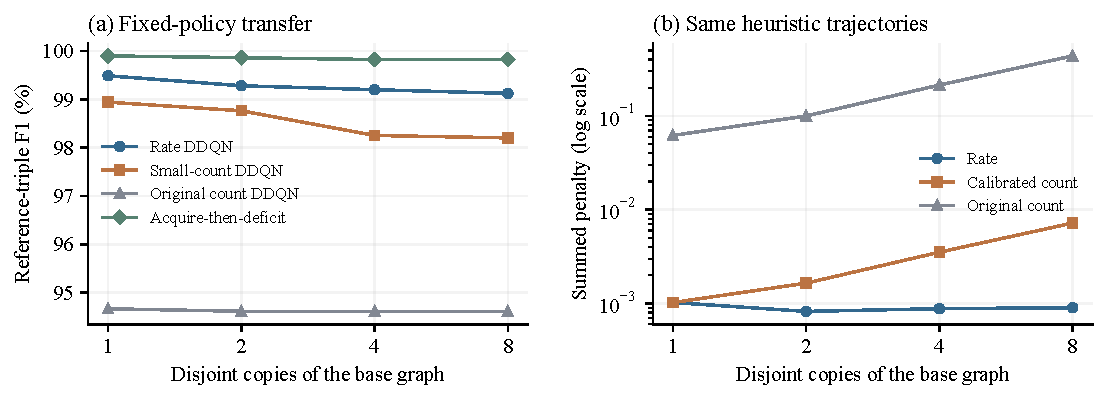
\includegraphics[width=0.94\textwidth]{figure/experiments/scale_control.pdf}

\caption{Graph-size test with disjoint copies. (a) Mean F1 across ten model seeds and five scenarios per size. (b) Three penalties on the same heuristic action logs. All models train at the base size.}

\label{fig:scale_control}

\end{figure*}

\begin{table}[t]

\centering

\caption{Heuristic time and memory, three runs per size. Time includes construction and actions with \texttt{tracemalloc}. Memory counts peak traced Python allocations during these steps. The clean graph and native tensor storage are excluded.}

\label{tab:scale_resources}

\scriptsize

\begin{tabular}{rrrr}

\toprule

Clean edges & Copies & Time (s) & Memory (MiB) \\

\midrule

1,083 & 1 & 0.881 & 1.32 \\

2,166 & 2 & 1.839 & 2.89 \\

4,332 & 4 & 4.126 & 5.46 \\

8,664 & 8 & 8.805 & 11.35 \\

\bottomrule

\end{tabular}

\end{table}

On the same heuristic action logs, the small-count burden grows by
7.06 times from one to eight copies. The rate burden changes by
0.88 times. These scores measure penalty scaling with matched actions.
